% LaTEX source code
% Last modified November 1st, 2005
% Steve Miller
% note that the percent sign comments out the rest of the line
% first, we set a document class. often use 12pt characters, though
% sometimes people do 11 or 10. you can do report or article, both similar
%\documentclass[12pt,letterpaper]{article}
\documentclass[12pt,reqno]{amsart}
\linespread{1}
\addtolength{\textwidth}{2cm} \addtolength{\hoffset}{-1cm}
\addtolength{\marginparwidth}{-1cm} \addtolength{\textheight}{2cm}
\addtolength{\voffset}{-1cm}
% below are some packages that are needed for certain symbols, graphics, colors.
% safest to just include these.
\usepackage{times}
\usepackage[T1]{fontenc}
\usepackage{mathrsfs}
\usepackage{latexsym}
\usepackage[dvips]{graphics}
\usepackage{epsfig}
\usepackage{hyperref, amsmath, amsthm, amsfonts, amscd, flafter,epsf}
\usepackage{amsmath,amsfonts,amsthm,amssymb,amscd}
\input amssym.def
\input amssym.tex
\usepackage{color}
\usepackage{enumerate}
\usepackage{hyperref}
\usepackage{url}
\usepackage{floatrow}
\usepackage{caption}
\usepackage{subcaption}
\usepackage{capt-of}
\usepackage{physics}
\newcommand{\todo}[1]{\textcolor{red}{\textbf{(#1)}}}

    %=======================================================

    %   THIS IS WHERE YOU PUT SHORTCUT DEFINITIONS

    %========================================================

% Note that we use a percent sign to comment out a line

% below are shortcut commands

%%%%%%%%%%%%%%%%%%%%%%%%%%%%%%%%%%%%%%%%%%%%%%%

% below are shortcuts for equation, eqnarray,

% itemize and enumerate environments

\newcommand\be{\begin{equation}}
\newcommand\ee{\end{equation}}
\newcommand\bea{\begin{eqnarray}}
\newcommand\eea{\end{eqnarray}}
\newcommand\bi{\begin{itemize}}
\newcommand\ei{\end{itemize}}
\newcommand\ben{\begin{enumerate}}
\newcommand\een{\end{enumerate}}
\newcommand{\ncr}[2]{\left({#1 \atop #2}\right)}
%%%%%%%%%%%%%%%%%%%%%%%%%%%%%%%%%%%%%%%%%%%%%%%%

% Theorem / Lemmas et cetera

\newtheorem{thm}{Theorem}[section]
\newtheorem{conj}[thm]{Conjecture}
\newtheorem{cor}[thm]{Corollary}
\newtheorem{lem}[thm]{Lemma}
\newtheorem{prop}[thm]{Proposition}
\newtheorem{exa}[thm]{Example}
\newtheorem{defi}[thm]{Definition}
\newtheorem{exe}[thm]{Exercise}
\newtheorem{rek}[thm]{Remark}
\newtheorem{que}[thm]{Question}
\newtheorem{prob}[thm]{Problem}
\newtheorem{cla}[thm]{Claim}
\newtheorem{defis}[thm]{Definitions}
\newtheorem{res}[thm]{Result}
\newtheorem{calc}[thm]{Calculation}
%%%%%%%%%%%%%%%%%%%%%%%%%%%%%%%%%%%%%%%%%

% shortcuts to environments

% this allows you to do textboldface: simply type \tbf{what you want in bold}

\newcommand{\tbf}[1]{\textbf{#1}}

%%%%%%%%%%%%%%%%%%%%%%%%%%%%%%%%%%%%%%%%%%%%%%%%%%

% shortcut to twocase and threecase definitions

\newcommand{\twocase}[5]{#1 \begin{cases} #2 & \text{#3}\\ #4
&\text{#5} \end{cases}   }
\newcommand{\threecase}[7]{#1 \begin{cases} #2 &
\text{#3}\\ #4 &\text{#5}\\ #6 &\text{#7} \end{cases}   }
%%%%%%%%%%%%%%%%%%%%%%%%%%%%%%%%%%%%%%%%%

%Blackboard Letters

\newcommand{\R}{\ensuremath{\mathbb{R}}}
\newcommand{\C}{\ensuremath{\mathbb{C}}}
\newcommand{\Z}{\ensuremath{\mathbb{Z}}}
\newcommand{\Q}{\mathbb{Q}}
\newcommand{\N}{\mathbb{N}}
\newcommand{\F}{\mathbb{F}}
\newcommand{\W}{\mathbb{W}}
\newcommand{\Qoft}{\mathbb{Q}(t)}  %use in linux
\newcommand{\soln}{\noindent \textbf{Solution:}\ }

%%%%%%%%%%%%%%%%%%%%%%%%%%%%%%%%%%%%%%%%%

% Finite Fields and Groups

\newcommand{\Fp}{ \F_p }
%%%%%%%%%%%%%%%%%%%%%%%%%%%%%%%%%%%%%%%%%

% Fractions

\newcommand{\foh}{\frac{1}{2}}  %onehalf
\newcommand{\fot}{\frac{1}{3}}
\newcommand{\fof}{\frac{1}{4}}

%%%%%%%%%%%%%%%%%%%%%%%%%%%%%%%%%%%%%%%%%

% Legendre Symbols

\newcommand{\js}[1]{ { \underline{#1} \choose p} }

%%%%%%%%%%%%%%%%%%%%%%%%%%%%%%%%%%%%%%%%%

% matrix shortcuts

\newcommand{\mattwo}[4]
{\left(\begin{array}{cc}
                        #1  & #2   \\
                        #3 &  #4
                          \end{array}\right) }
\newcommand{\matthree}[9]
{\left(\begin{array}{ccc}
                        #1  & #2 & #3  \\
                        #4 &  #5 & #6 \\
                        #7 &  #8 & #9
                          \end{array}\right) }
\newcommand{\dettwo}[4]
{\left|\begin{array}{cc}
                        #1  & #2   \\
                        #3 &  #4
                          \end{array}\right| }
\newcommand{\detthree}[9]
{\left|\begin{array}{ccc}
                        #1  & #2 & #3  \\
                        #4 &  #5 & #6 \\
                        #7 &  #8 & #9
                          \end{array}\right| }
%%%%%%%%%%%%%%%%%%%%%%%%%%%%%%%%%%%%%%%%%

% greek letter shortcuts

\newcommand{\ga}{\alpha}                  %gives you a greek alpha
\newcommand{\gb}{\beta}
\newcommand{\gep}{\epsilon}
%%%%%%%%%%%%%%%%%%%%%%%%%%%%%%%%%%%%%%%%%

% general functions

\newcommand{\notdiv}{\nmid}               % gives the not divide symbol
\newcommand{\burl}[1]{\textcolor{blue}{\url{#1}}}

%%%%%%%%%%%%%%%%%%%%%%%%%%%%%%%%%%%%%%%%%%%

% the following makes the numbering start with 1 in each section;

% if you want the equations numbered 1 to N (without caring about

% what section you are in, comment out the following line.

\numberwithin{equation}{section}

%\textwidth= 6in

%\evensidemargin=37pt

%\oddsidemargin=0pt

\begin{document}



\title{Hexane Water Results Log}
\author{Kirk Swanson}
\email{swansonk1@uchicago.edu}
\address{Institute for Molecular Engineering, University of Chicago, 5640 S Ellis Ave, Chicago, IL 60637}
%\keywords{path integral molecular dynamics, path integral monte carlo, metropolis algorithm}
\date{\today}




\maketitle

%%%%%%%%%%%%%%%%%%%%%%%%%%%%%%%%%%%%%%%%%%%%%%%%%%%%%%%%%%%%%%%%%%%%%%%%%%%%%%%%%%%%%%%%%%%%%%%%%%%%%%%%%%%%%%%%%%%%%%%%%%%%%%

\normalsize

%%%%%%%%%%%%%%%%%%%%%%%%%%%%%%%%%%%%%%%%%%%%%%%%%%%%%%%%%%%%%%%%%%%%%%%%%%%%%%%%%%%%%%%%%%%%%%%%%%%%%%%%%%%%%%%%%%%%%%%%%%%%%%

\section{1/8/2018}
\begin{enumerate}
\item Ran a simulation of the hexane-water interface using LAMMPS.  Set up for 1M time steps, but only got through 745,200 due to time limit of 24 hrs.  
\item Ran a simulation of the hexane-water interface in DASH, using the python script "interface.py" in the dash-work/interface folder.  The run was for 4,000,000 time steps, printing a configuration every 50,000 steps.  Below are snapshots of the 0th timestep and the 3,950,000 time step.    

\begin{figure}[H]
\centering
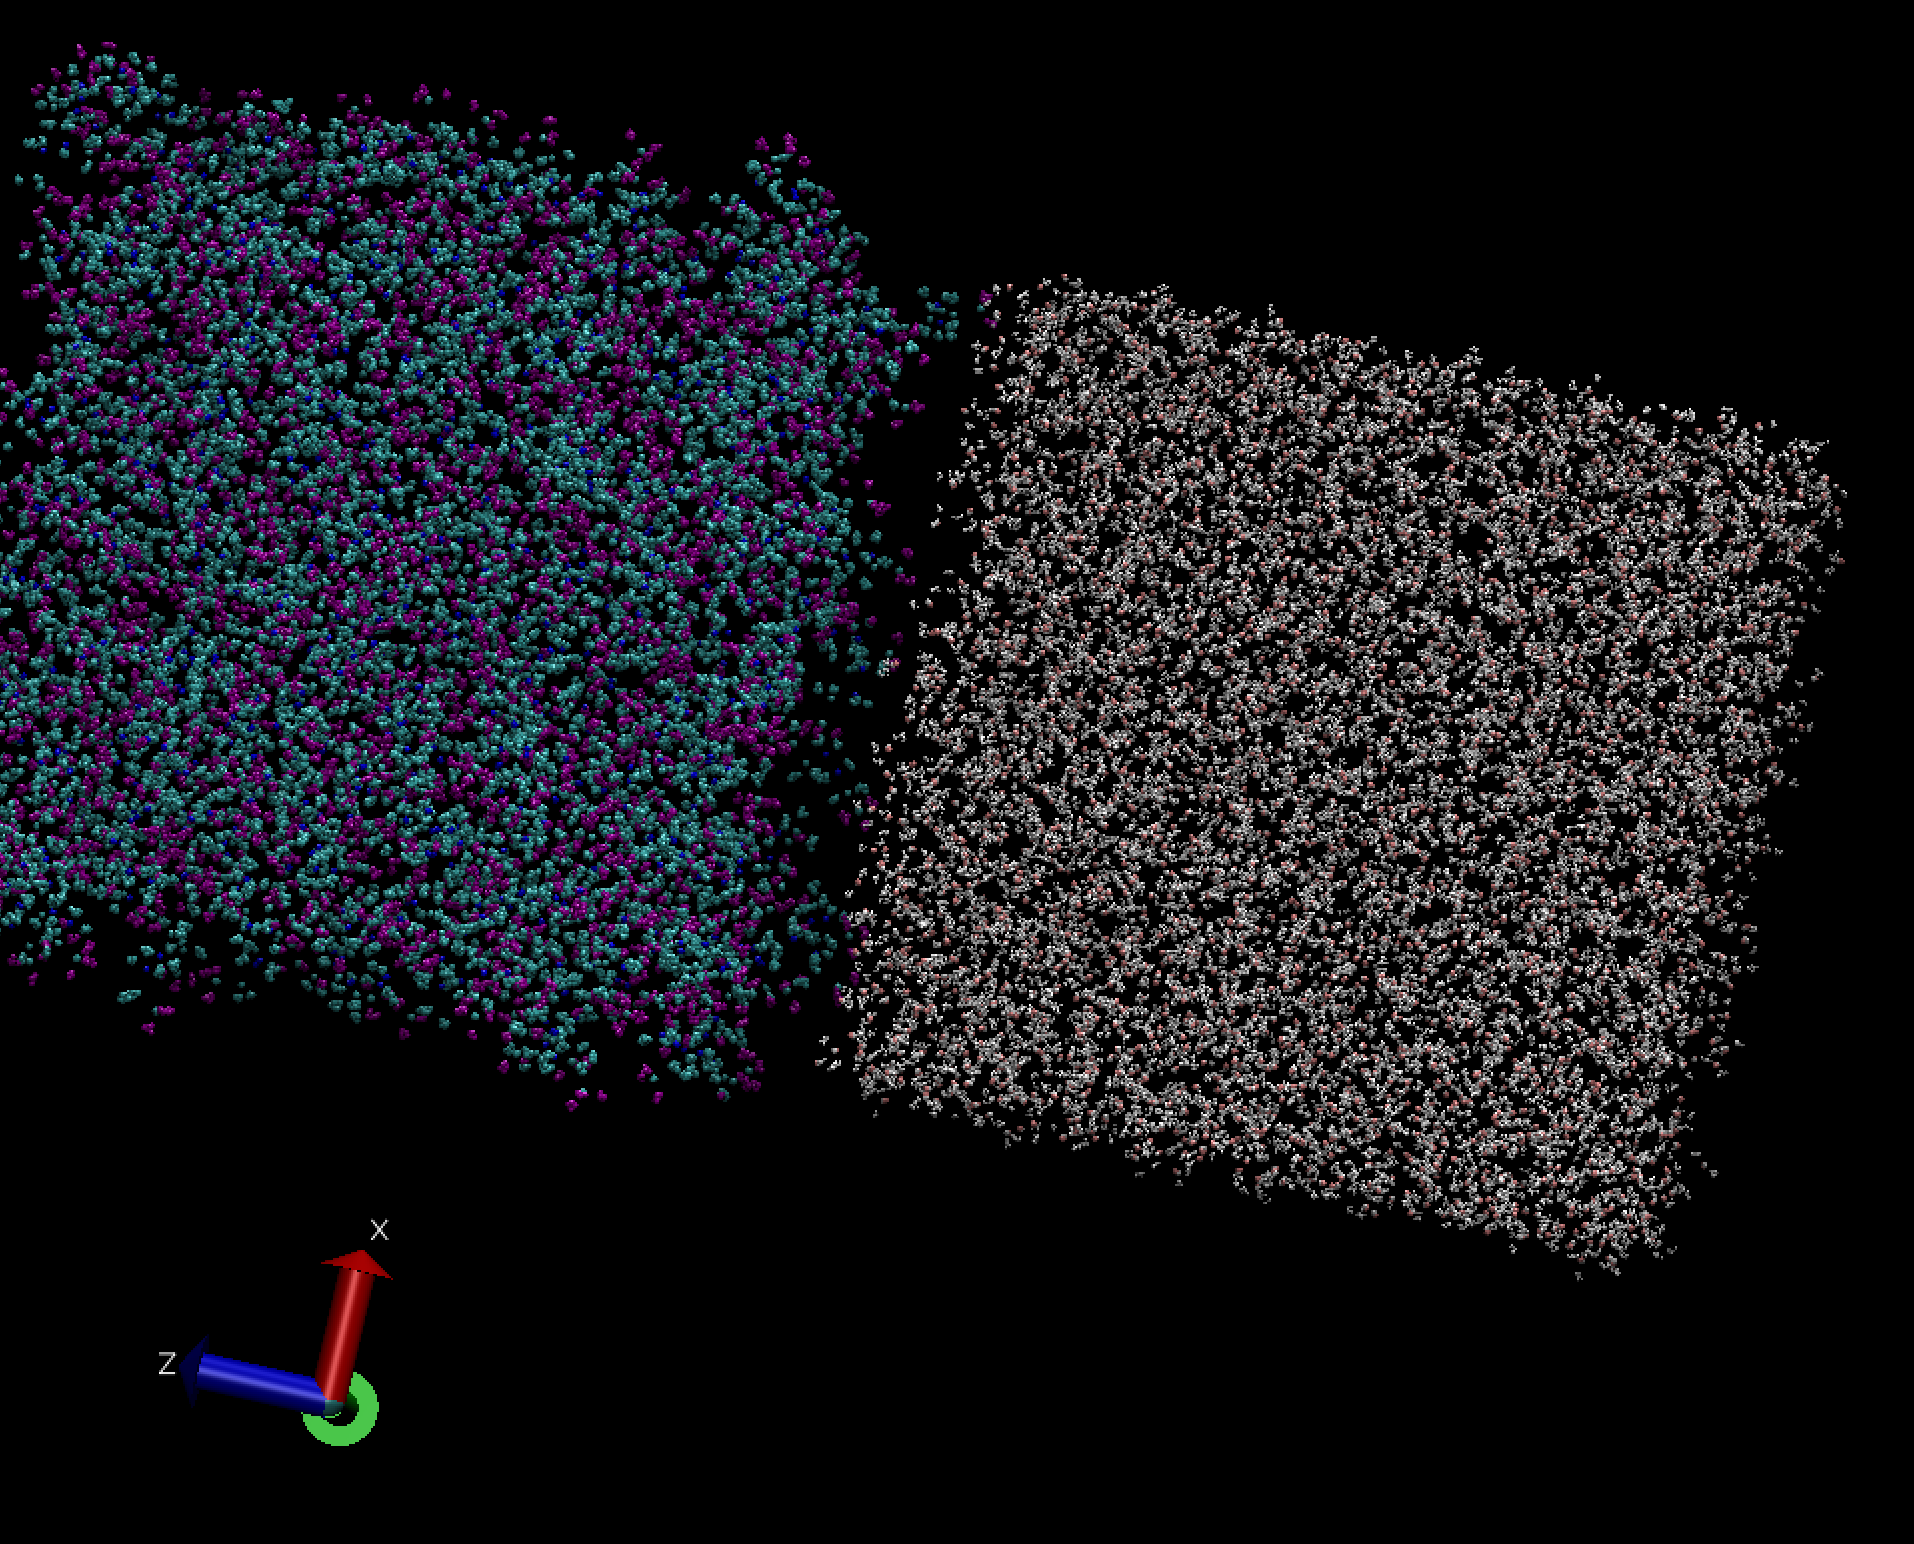
\includegraphics[scale=0.4]{dash_taffi-tip4pF_8beads_0}
\caption{DASH simulation of the TAFFI - q-TIP4P/F interface.  Arithmetic mixing, 4,000,000 time steps.  This is the 0th timestep.}
\end{figure}

\begin{figure}[H]
\centering
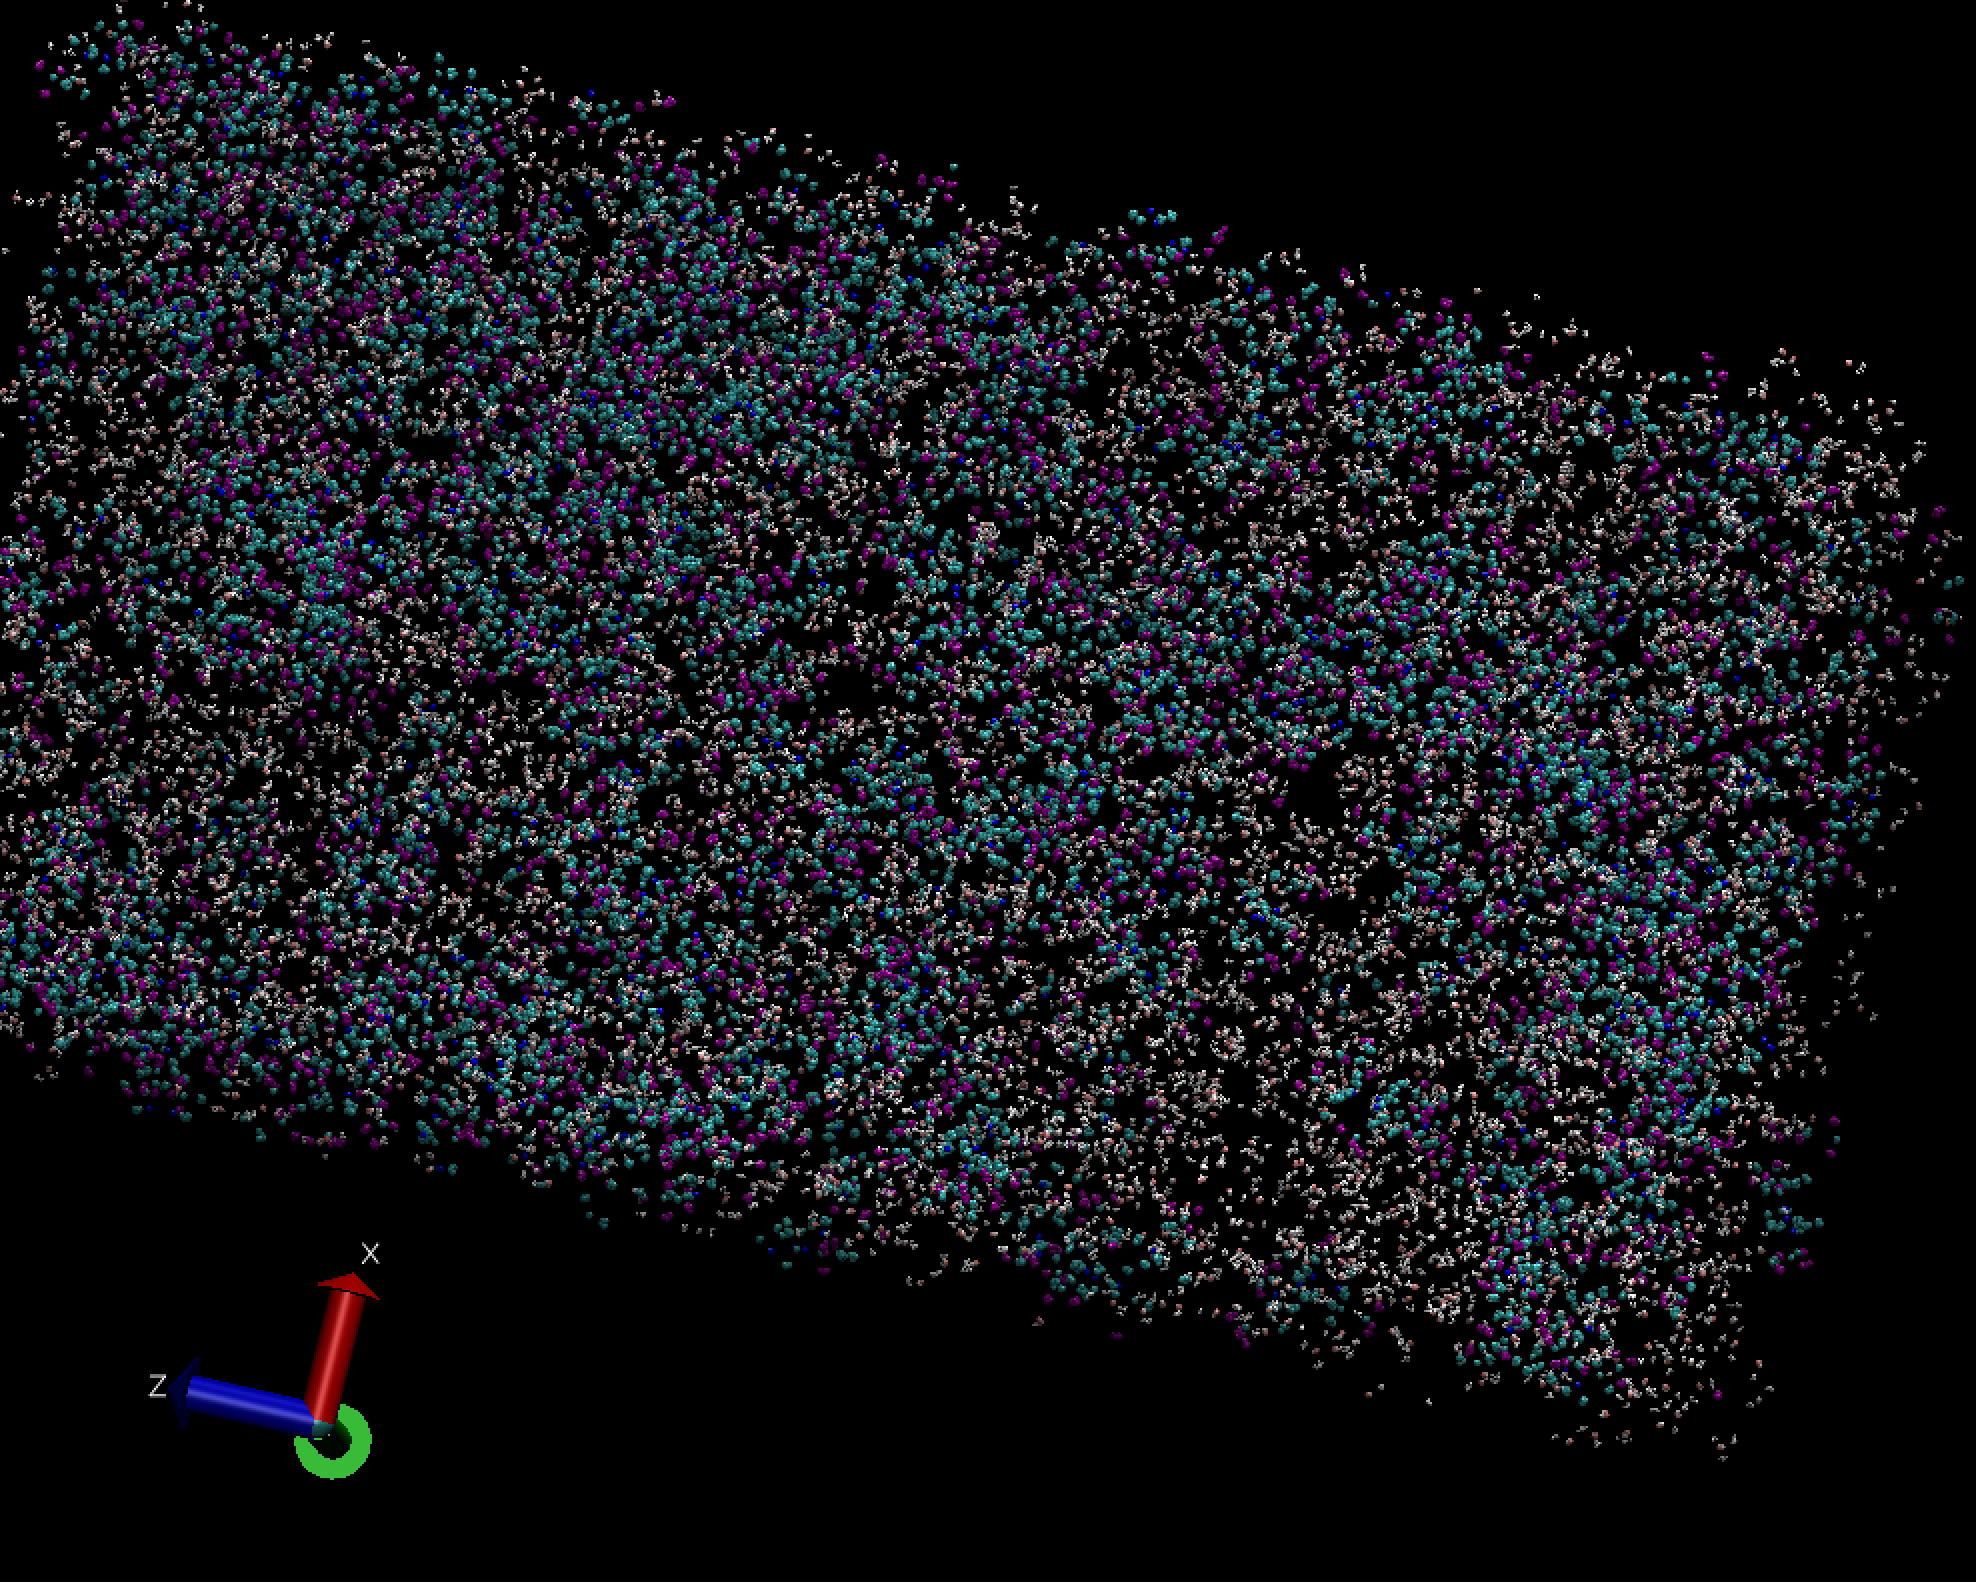
\includegraphics[scale=0.4]{dash_taffi-tip4pF_8beads_3950000}
\caption{DASH simulation of the TAFFI - q-TIP4P/F interface.  Arithmetic mixing, 4,000,000 time steps.  This is the 3,950,000th timestep.}
\end{figure}

\item This is in stark contrast to the amount of mixing that we observed in OPLS + TIP4P/2005 in LAMMPS, which was the appropriate amount of mixing, i.e., very little mixing.  So, there are several possible things going on here.  One is that there is an error in the code.  Another is that there is an error in DASH.  And third is that there is a problem with the interaction parameters between the two force fields.  So, here are the following tests that we are going to run to narrow down the problem:
\subitem Run TAFFI + TIP4P/F in LAMMPS using arithmetic, geometric, and Waldman-Hagler mixing rules and using both TAFFI and OPLS parameters for hexane 
\subitem Run TAFFI + TIP4P/F in DASH using geometric and Waldman-Hagler mixing rules using both TAFFI and OPLS parameters and using 1 bead versus 8 beads
\subitem Run OPLS + TIP4P/F in DASH using geometric mixing rules and using 1 bead versus 8 beads
\subitem Check for any errors in the DASH input scripts
\subitem TAFFI + TIP4P/F in DASH using on bead

\item So, the first step we are going to take is to run TAFFI + q-TIP4P/F in LAMMPS using arithmetic mixing rules.  Let's first take a look at the simulation of TAFFI + TIP4P/2005 and see what that snapshot looks like.  At timestep zero:

\begin{figure}[H]
\centering
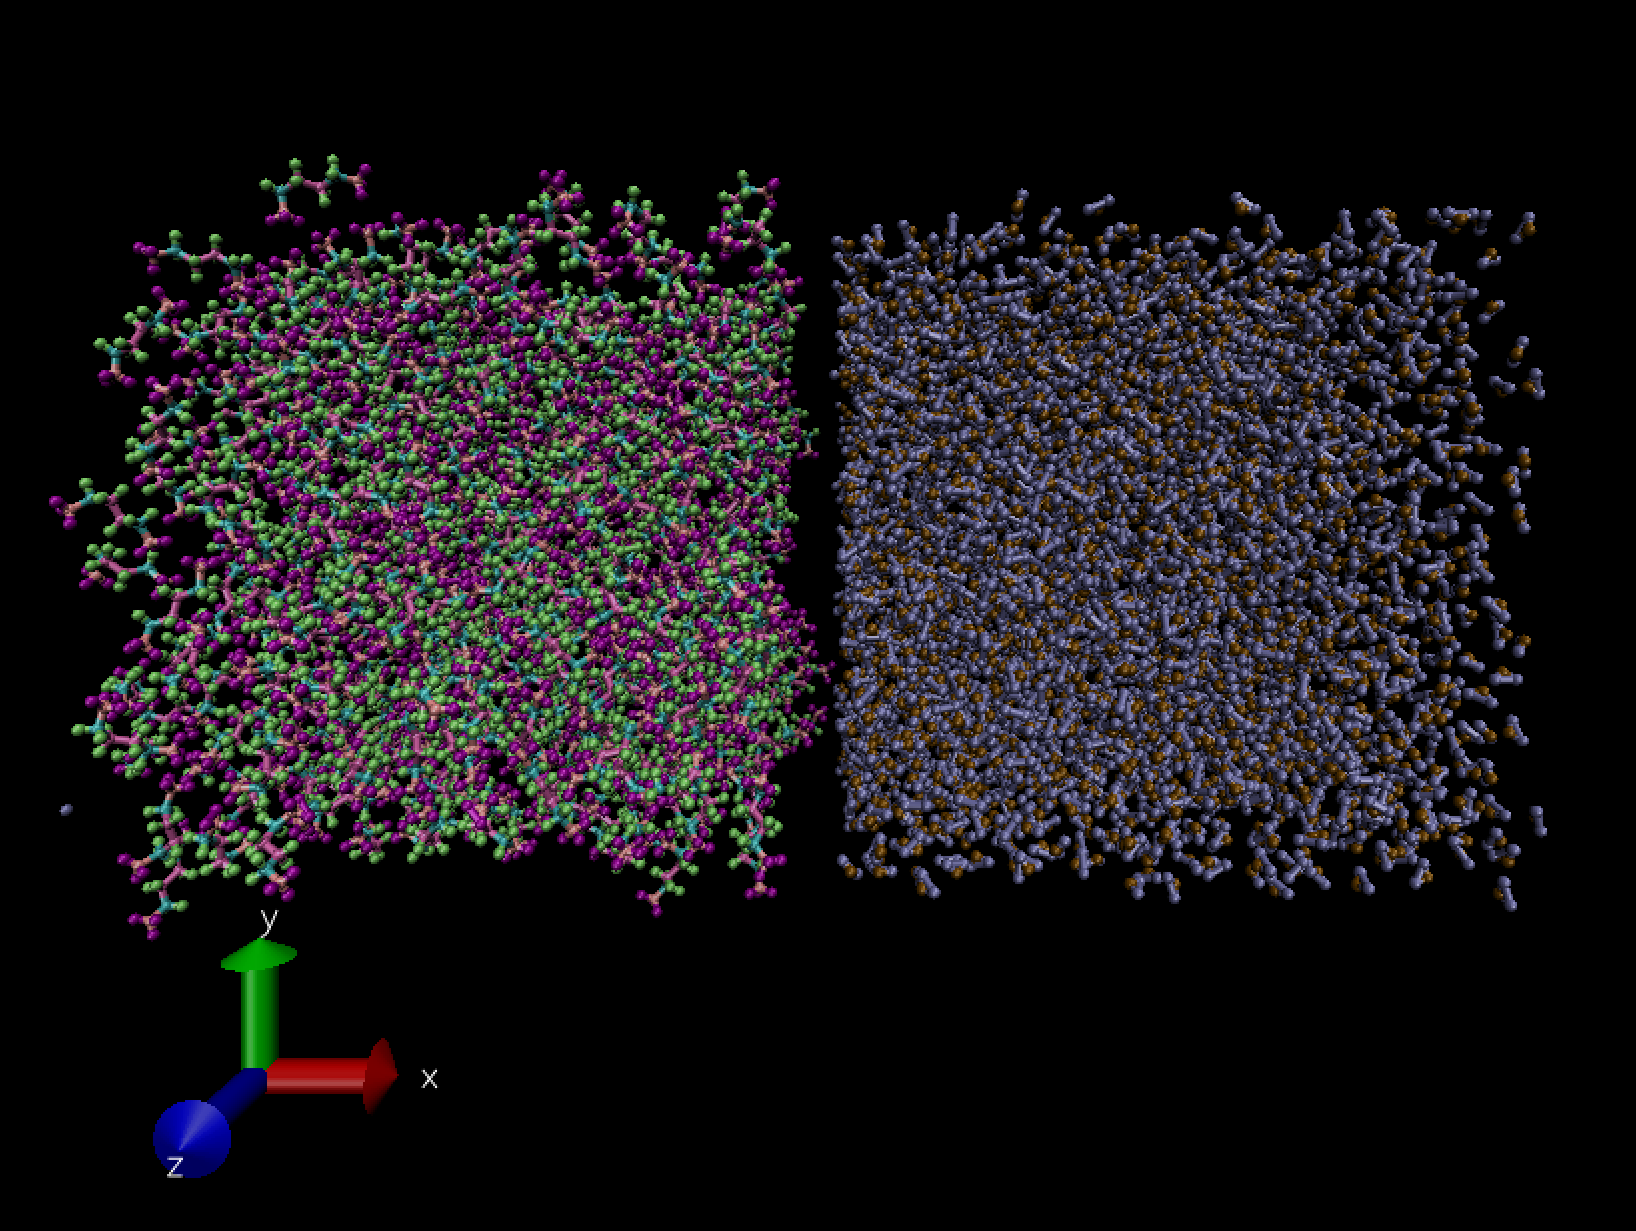
\includegraphics[scale=0.4]{lammps_taffi-tip4p2005_0}
\caption{Lammps simulation of the TAFFI - TIP4P/2005 interface.  Arithmetic mixing, 200,000 time steps.  This is the 0th timestep.}
\end{figure}

After 200,000 time steps:

\begin{figure}[H]
\centering
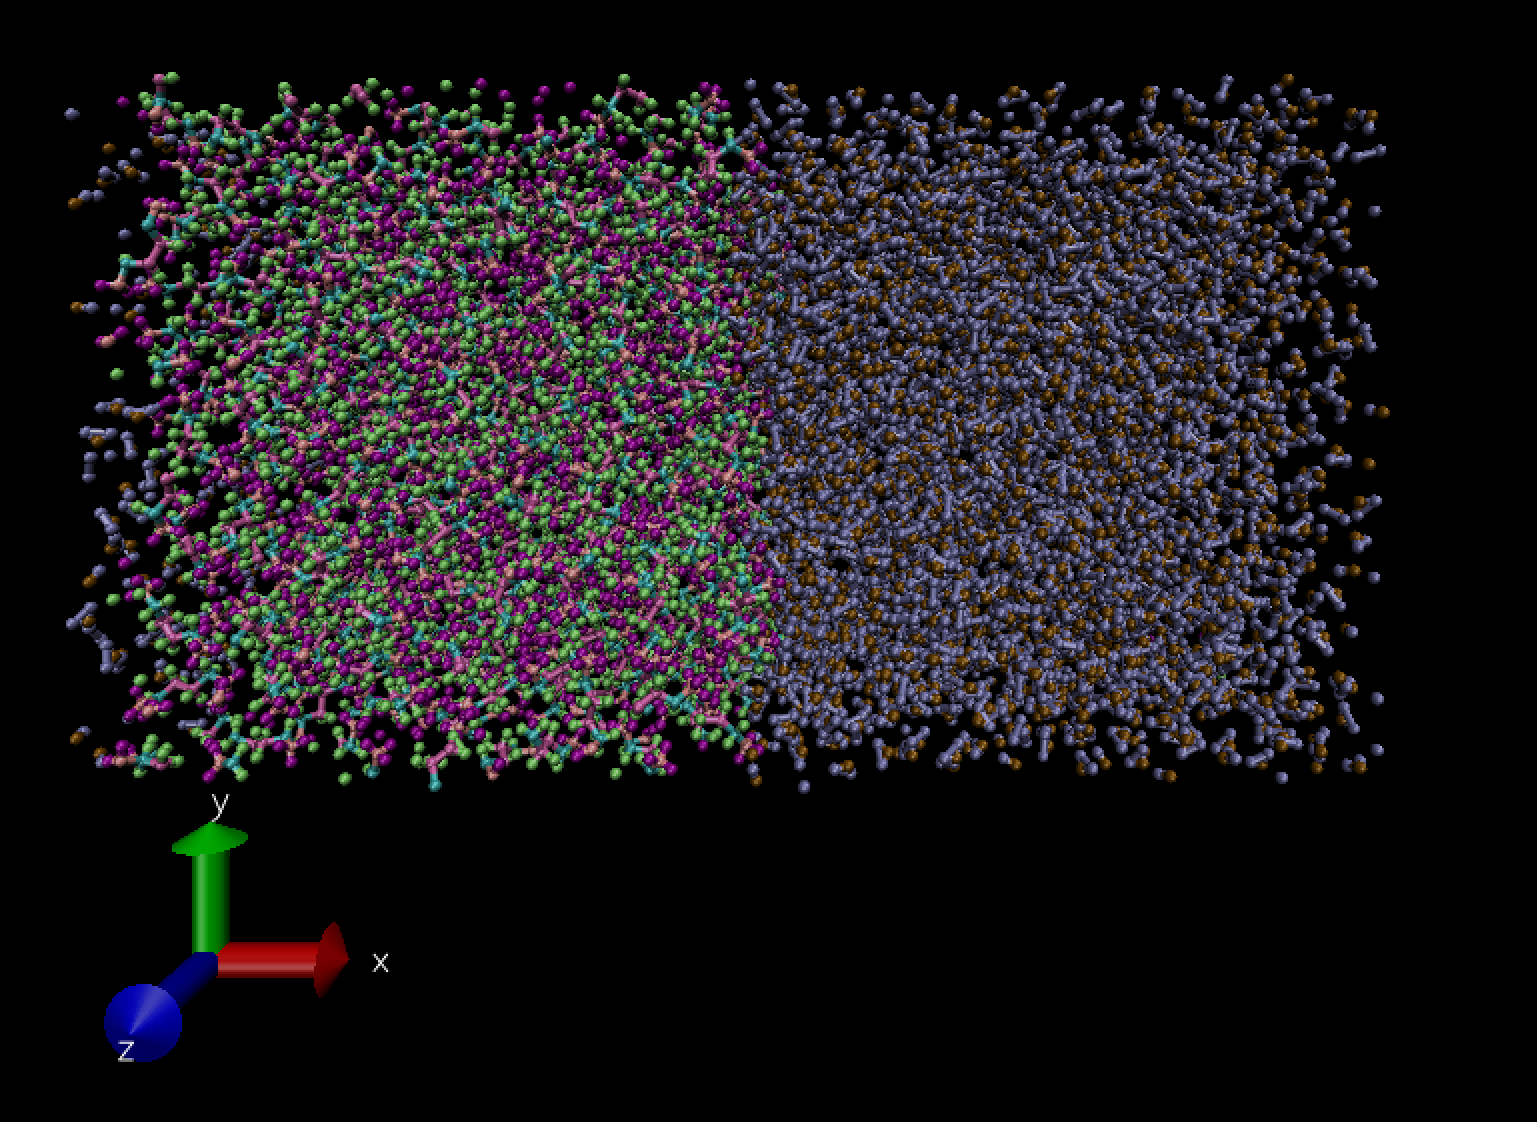
\includegraphics[scale=0.4]{lammps_taffi-tip4p2005_200000}
\caption{Lammps simulation of the TAFFI - TIP4P/2005 interface.  Arithmetic mixing, 200,000 time steps.  This is the 199,000th timestep.}
\end{figure}

For more direct comparison, here is the dash version of TAFFI + TIP4P/F at 200,000 steps:

\begin{figure}[H]
\centering
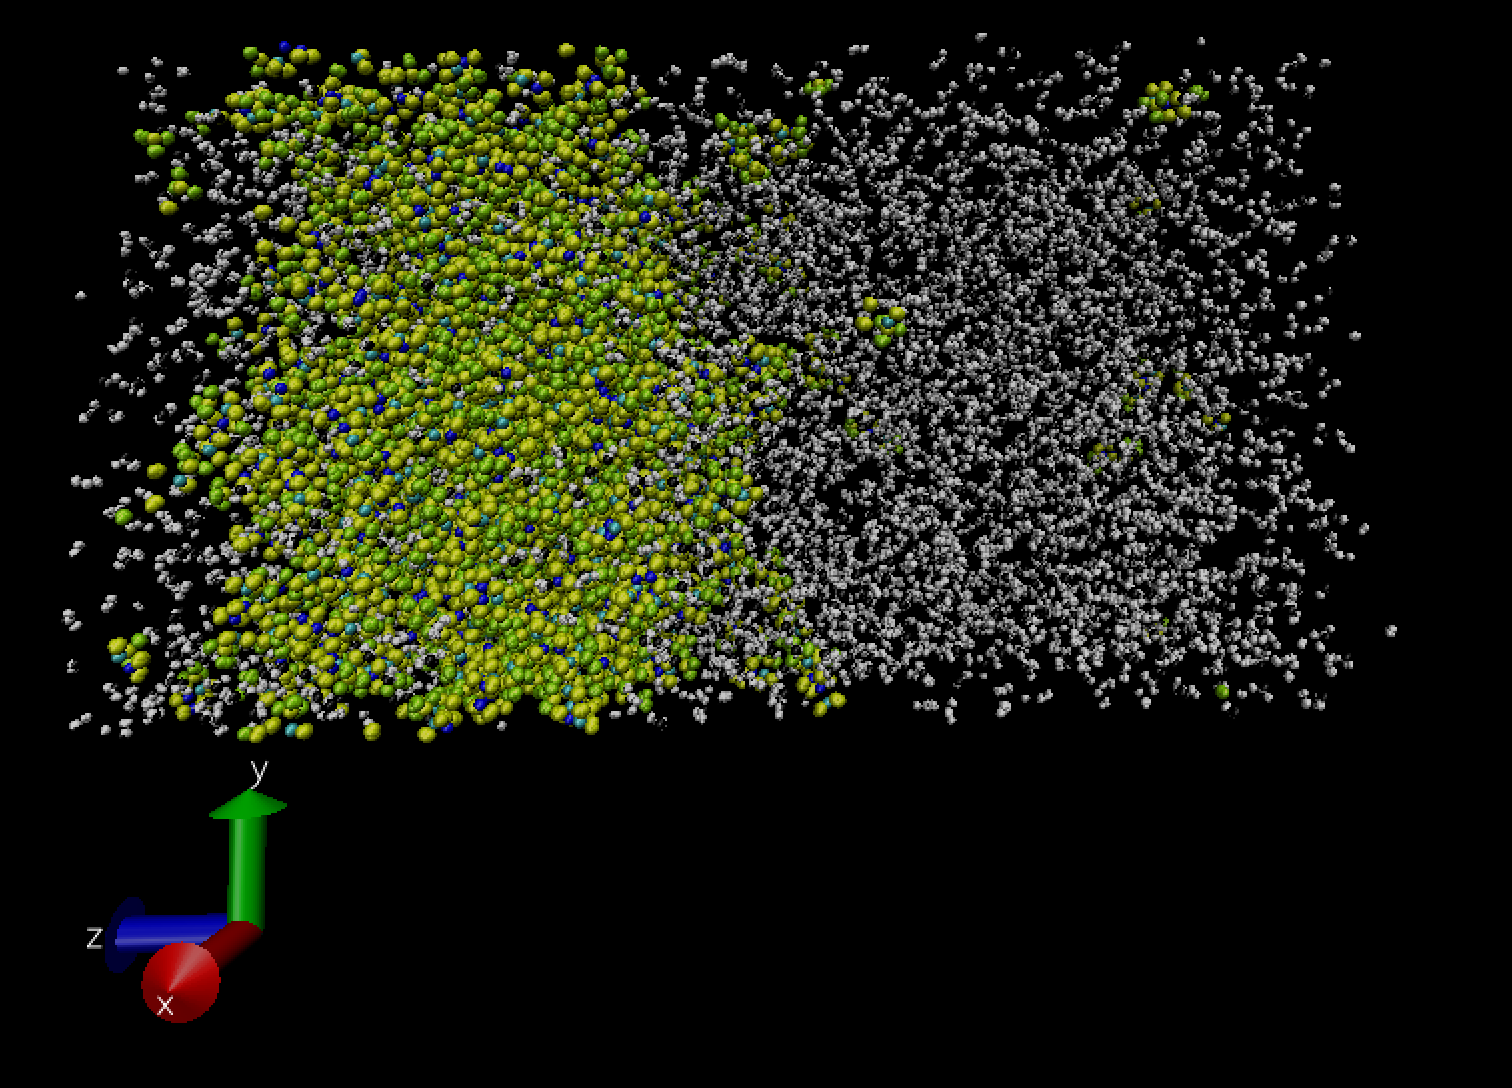
\includegraphics[scale=0.4]{dash_taffi-tip4pF_8beads_200000}
\caption{DASH simulation of the TAFFI - q-TIP4P/F interface.  Arithmetic mixing, 4,000,000 time steps.  This is the 3,950,000th timestep.}
\end{figure}

\item Now, we are going to construct the TIP4P/F in LAMMPS.  The starting point is the TIP4P/2005 classical rigid water model, which we have already implemented.  The next step is to add a quartic expansion of a Morse potential for the OH stretch:
\begin{align}
\begin{split}
V_{OH}(r) = D_r\left[\alpha_r^2(r - r_0)^2 - \alpha_r^3(r - r_0)^3 + \frac{7}{12}\alpha_r^4(r - r_0)^4\right], 
\end{split}
\end{align}
where $D_r = 116.09$, $\alpha_r = 2.287$, and $r_0 = 0.9419$.  

And then we add a simple harmonic potential for the bond angle:

\begin{align}
\begin{split}
V_{HOH}(\theta) = \frac{1}{2}k_\theta(\theta - \theta_0)^2, 
\end{split}
\end{align}
where $k_\theta = 87.85$, and $\theta_0 = 107.4$.


\item In LAMMPS, then, we will try using bond\_style class2 for the quartic expansion of the Morse potential for the OH stretch:

\begin{align}
\begin{split}
E = K_2(r - r_0)^2 + K_3(r - r_0)^3 + K_4(r - r_0)^4,
\end{split}
\end{align}
where $r_0 = r_{eq}$, $K_2 = \alpha_r^2 = 5.23$, $K_3 = -\alpha_r^3 = -11.962$, and $K_4 = \frac{7}{12}\alpha_r^4 = 15.958$.

\item We will use angle\_style harmonic for the simple harmonic potential for the bond angle:

\begin{align}
\begin{split}
E = K(\theta - \theta_0)^2,
\end{split}
\end{align}
where $K = \frac{1}{2}k_\theta$ and $\theta_0 = \theta_{eq} = 107.4$.  

\item Then, we created a data\_water\_flexible.txt file, which is a data file describing a single TIP4P/F water molecule for lammps.  I then created an in.water\_flexible file, a lammps input file to run the flexible water model simulation.  I modified this from the TIP4P/2005 input file by removing the fix shake command and adding the bond\_style class2 command.  I then ran lammps\_molecule\_replicator\_water.py in order to get 3650 flexible water molecules on an initial lattice.  
\item I tried running a lammps simulation using in.water\_flexible, but I am getting the error that the program does not recognize class2.  Turns out that this belongs to the LAMMPS package CLASS2, which might not be compiled for in my folder.  So checking that now.  

\item Compiled LAMMPS with CLASS2, and now able to run the flexible water model.  However, massive forces seem to be appearing as I am getting the error: "Out of range atoms - cannot compute PPPM).  It works better if I make the timestep miniscule, but it still breaks eventually.  Sometimes says missing bonds or atoms.  My guess is that I shouldn't be using the command pair\_style lj/cut/tip4p/long.  So perhaps for next time, what I need to do is just implement the water model irrespective of that particular pair style command, and instead I need to input all of the specifications by hand.  

\item Setting that aside for now, let's turn to DASH again, and try different parameter sets here.  Let's first work just in the classical world, with one bead.  First, let's run TAFFI + TIP4P/F in DASH using TAFFI parameters, geometric mixing, and 1 bead.   
\item This is currently running.
\item Now, let's run TAFFI + TIP4P/F in DASH using TAFFI parameters, arithmetic mixing, and 1 bead.  Just to check/be consistent.  
\item This is also currently running.  

 

\end{enumerate}

\subsection{2/23/2018}
\begin{enumerate}
\item NOTICED AN ERROR: MISSING FACTOR OF 116 IN THE BOND POTENTIAL.  FIX THIS NEXT. 
\end{enumerate}

\subsection{2/27/2018}
\begin{enumerate}
\item Fixed this problem, added the missing factor of 166.09 in the bond potential where it was due.  Saved the resulting new input file.  Currently, running an NPT system of 3650 water molecules in order to generate an initial configuration for the test interface of q-TIP4P/F and TAFFI in LAMMPS.  
\item The TAFFI + TIP4P/F in DASH using TAFFI parameters, arithmetic mixing, and 1 bead finished running.  There is too much mixing going on.  Here is a snapshot at time zero:

\begin{figure}[H]
\centering
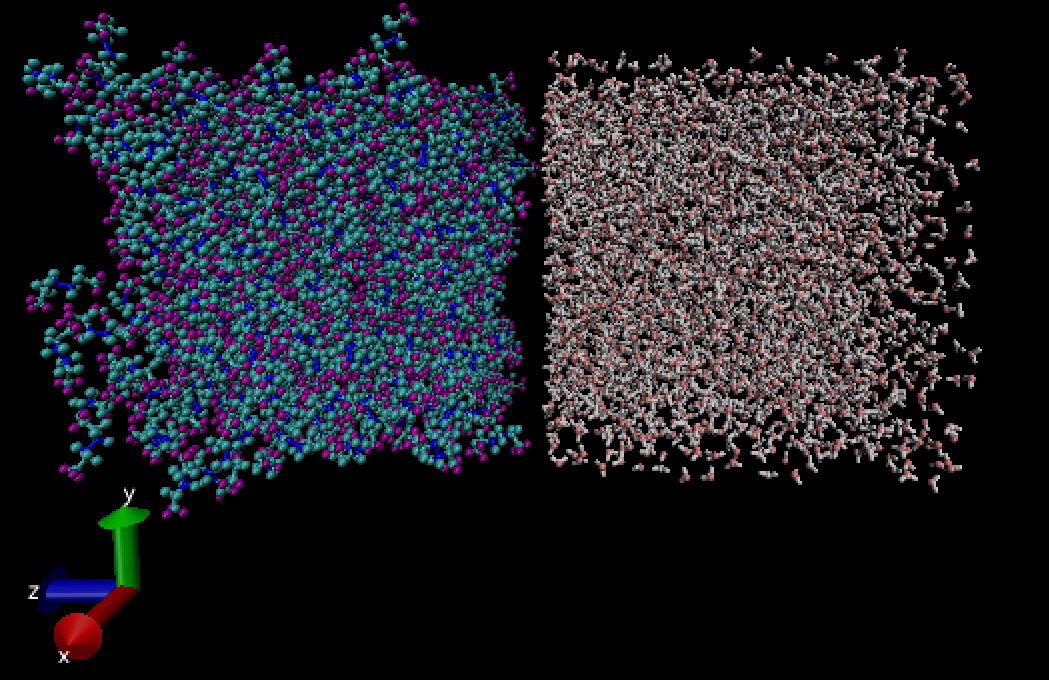
\includegraphics[scale=0.7]{dash_taffi-tip4pF_arithmetic_1bead_0}
\caption{DASH simulation of the TAFFI - q-TIP4P/F interface.  Arithmetic mixing, 4,000,000 time steps, 1 bead.  This is the 0th timestep.}
\end{figure}

\item Here is a snapshot after 4,000,000 timesteps of length 0.5:
\begin{figure}[H]
\centering
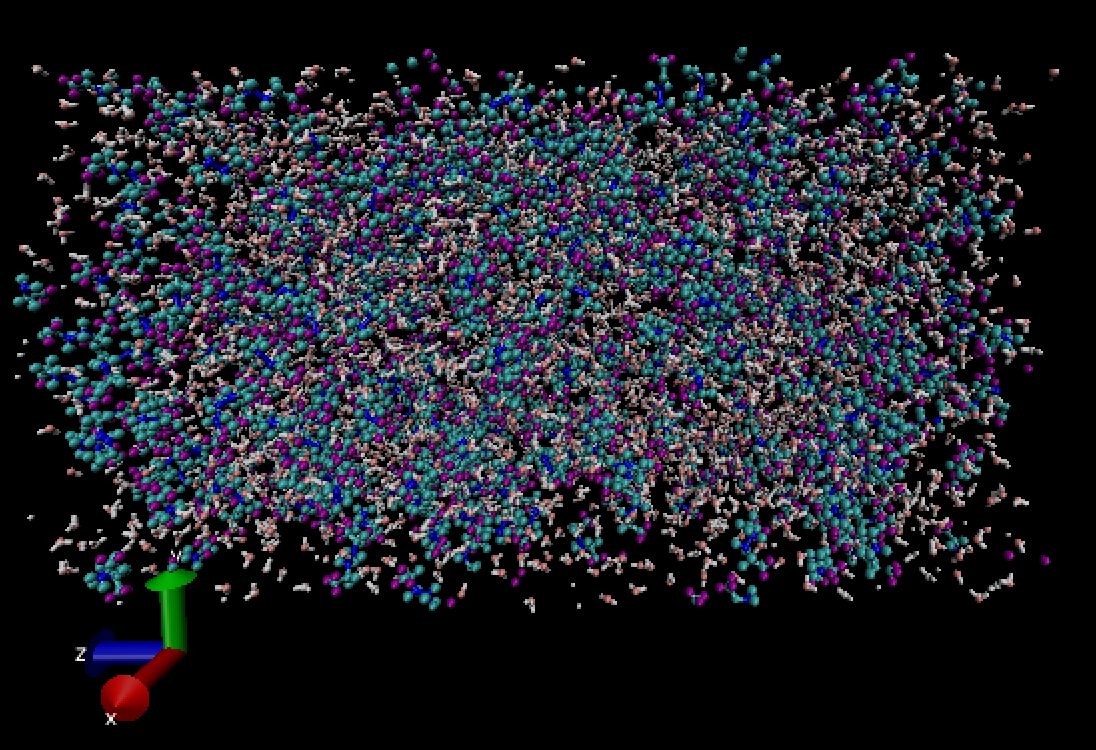
\includegraphics[scale=0.7]{dash_taffi-tip4pF_arithmetic_1bead_3950000}
\caption{DASH simulation of the TAFFI - q-TIP4P/F interface.  Arithmetic mixing, 4,000,000 time steps, 1 bead.  This is the 3950000th timestep.}
\end{figure}

\item The TAFFI + TIP4P/F in DASH using TAFFI parameters, geometric mixing, and 1 bead also finished running.  There is too much mixing.  Here is a snapshot at time zero:

\begin{figure}[H]
\centering
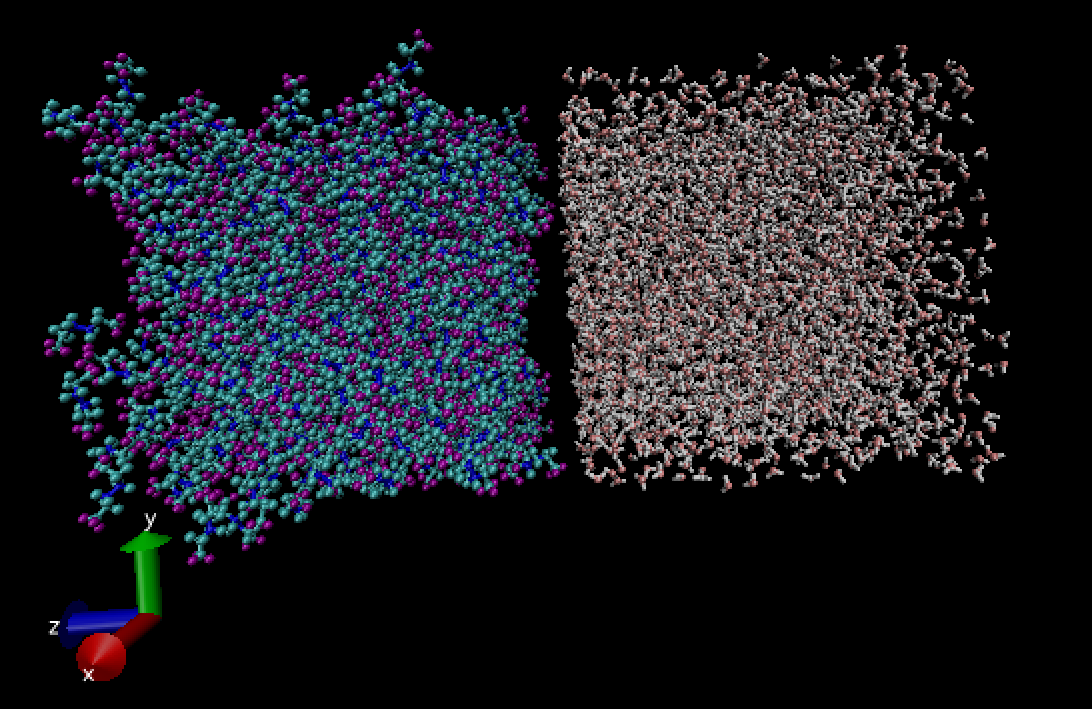
\includegraphics[scale=0.7]{dash_taffi-tip4pF_geometric_1bead_0}
\caption{DASH simulation of the TAFFI - q-TIP4P/F interface.  Geometric mixing, 4,000,000 time steps, 1 bead.  This is the 0th timestep.}
\end{figure}

\item Here is after 4,000,000 timesteps of length 0.5:

\begin{figure}[H]
\centering
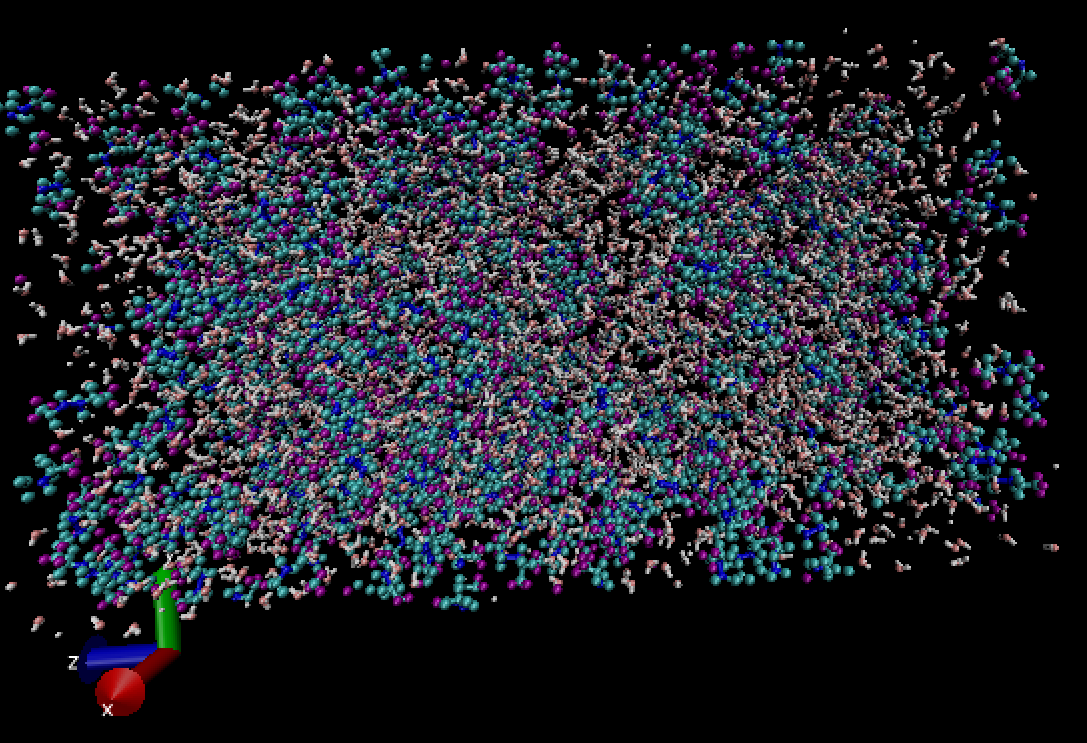
\includegraphics[scale=0.7]{dash_taffi-tip4pF_geometric_1bead_3950000}
\caption{DASH simulation of the TAFFI - q-TIP4P/F interface.  Geometric mixing, 4,000,000 time steps, 1 bead.  This is the 0th timestep.}
\end{figure}


  
\end{enumerate}

\end{document}

%%%%%%%%%%%%%%%%%%%%%%%%%%%%%%%%%%%%%%%%%%%%%%%%%%%%%%%%%%%%%%%%%%%%%%%%%%%%%%%%%%%%%%%%%%%%%%%%%%%%%%%%%%%%%%%%%%%%%%%%%%%%%%